\section{Extreme Programming}

La metodología utilizada ha sido eXtreme Programming (XP en adelante). Esto es debido a que es una
metodología iterativa-incremental la cual permite el desarrollo de aplicaciones de modo que en cada
iteración aumente la funcionalidad de la misma. Una de las principales ventajas que nos ofrece
es su cercanía a la improvisación. Como se dijo antes necesitaremos una metodología la cual
nos permita improvisar, puesto que desconocemos el camino a seguir. XP también nos facilita
el incremento de funcionalidades con el paso del tiempo, puesto que se centra en sacar versiones
estables del proyecto y no pasar a la siguiente hasta que no este estable. En la \hyperref[fig:Desarrollo Sistema Experto]{figura 4.1} se
puede ver el flujo normal trabajando con extreme programming


\begin{figure}[htb]
  \centering
    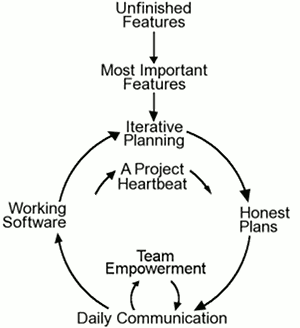
\includegraphics[width=0.4\linewidth]{agileflowchart}
  \caption[Desarrollo SE]{Desarrollo SE}
  \label{fig:Desarrollo Sistema Experto}
\end{figure}



\subsection{Valores}

Los valores que se defienden en esta metodología son los siguientes:

\begin{itemize}
  \item \textbf{Simplicidad:} Esta es la base de XP. Cuanto mas simple sea el diseño, mas sencillo será de programarlo. Es por esto
    por lo que deberemos tener especial atención a las definiciones de los problemas. Para ayudar a un código sencillo se facilitará
    la refactorización de código cuanto sea necesario en cada iteración. De este modo no generaremos un código muy complejo según
    añadamos funcionalidades. La documentación del código no deberá ser muy extensa ya que un buen código estará auto documentado
    y se entenderá por si mismo.
  \item \textbf{Comunicación:} Reforzando el anterior apartado, la comunicación ha de ser sencilla. Evitar los comentarios
    en el código y mejorar este para que se explique automáticamente es algo fundamental. Por otro lado el desarrollo
    de test unitarios facilita la comunicación, puesto que estos explicarán de una manera muy clara los casos de uso.
  \item \textbf{Retroalimentación:} En esta metodología el cliente está muy implicado. Los tiempos en los que se hacen
    desarrollo y se entrega al cliente son muy cortos, de modo que se pueden comprobar funcionalidades poco después
    de desarrollarlas. De este modo evitaremos en gran medida los desarrollos que después de enseñárselos al cliente se desechan.
  \item \textbf{Valentía:} Para esta metodología tenga éxito hay que ser valiente tomando decisiones para que el diseño no se complique
    demasiado, puesto que esto conllevaría mayor tiempo de desarrollo, lo cual haría verse comprometida la faceta de entregas
    en poco tiempo.
  \item \textbf{Respeto:} Todos los miembros del equipo han de ser respetados. Todos los miembros del equipo aportan
    algo a él y no funcionaría sin ellos. Desde la dirección se respetará a dar responsabilidades a cada uno de los miembros.
\end{itemize}

\subsection{Características}

Lo que caracteriza a esta metodología es lo siguiente:

% Cambiar las palabras de esto
\begin{itemize}
  \item \textbf{Desarrollo iterativo e incremental:} pequeñas mejoras, unas tras otras.
  \item \textbf{Pruebas unitarias continuas,} frecuentemente repetidas y automatizadas, incluyendo pruebas de regresión. Se aconseja escribir el código de la prueba antes de la codificación. Véase, por ejemplo, las herramientas de prueba JUnit orientada a Java, DUnit orientada a Delphi, NUnit para la plataforma.NET o PHPUnit para PHP. Estas tres últimas inspiradas en JUnit, la cual, a su vez, se insipiró en SUnit, el primer framework orientado a realizar tests, realizado para el lenguaje de programación Smalltalk.equeñas mejoras, unas tras otras.
  \item \textbf{Programación en parejas:} se recomienda que las tareas de desarrollo se lleven a cabo por dos personas en un mismo puesto. La mayor calidad del código escrito de esta manera -el código es revisado y discutido mientras se escribe- es más importante que la posible pérdida de productividad inmediata. Esta característica no podrá ser cumplida puesto que el desarrollo lo realizará una única persona.
  \item \textbf{Integración del equipo de programación con el cliente o usuario.} Se recomienda que un representante del cliente trabaje junto al equipo de desarrollo.
  \item \textbf{Corrección de todos los errores} antes de añadir nueva funcionalidad. Hacer entregas frecuentes.
  \item \textbf{Refactorización del código} reescribir ciertas partes del código para aumentar su legibilidad y mantenibilidad pero sin modificar su comportamiento. Las pruebas han de garantizar que en la refactorización no se ha introducido ningún fallo.
  \item \textbf{Propiedad del código compartida:} en vez de dividir la responsabilidad en el desarrollo de cada módulo en grupos de trabajo distintos, este método promueve el que todo el personal pueda corregir y extender cualquier parte del proyecto. Las frecuentes pruebas de regresión garantizan que los posibles errores serán detectados.
  \item \textbf{Simplicidad en el código: } es la mejor manera de que las cosas funcionen. Cuando todo funcione se podrá añadir funcionalidad si es necesario. La programación extrema apuesta que es más sencillo hacer algo simple y tener un poco de trabajo extra para cambiarlo si se requiere, que realizar algo complicado y quizás nunca utilizarlo.
\end{itemize}
